%kelompok 1 Sistem Operasi (Proses Os)
%Kelas D4 TI 1B
%Adam Noer Hidayatullah 1174097
%Ichsan Hizman
%Teddy
%Nisrina Aulia
%Irvan Rizkiansyah 1174043

\section{PIP}

    \subsection{PIP}
	PIP adalah singkatan dari pip installs python.sebuah tool yang memudahkan programmer untuk menginstall library-library  atau disebut juga sebuah package manager untuk Python

	\subsection{cara install pip di windows}
	Sebelum melakukan peng-install-an pip, di wajibkan untuk menginstall python terlebih dahulu. Karena tanpa python tidak akan bisa mengeksekusi installer pip, dan pastikan environment variables python nya sudah ter-setting
		\begin{enumerate}
			\item download pip langsung ke website resminya di \url{<https://pip.pypa.io/en/latest/installing/>}
			\item letakan file get-pip.py ke direktori yang mudah di temukan.
			\item Buka CMD dan masuk ke direktori file get-pip.py yang tadi sudah diletakkan direktori.
			\item Pada saat di CMD langsung ketikkan python get-pip.py .
			\item tunggu proses nya hingga selesai.
			\item Setelah menginstall, kini saatnya mensetting Environment Variables supaya mudah dan dapat menjalankan pip lewat CMD tanpa harus masuk ke dalam folder hasil instalasi pip.
			\item Masuk ke dalam Control Panel - System And Security - System - advanced System Settings
			\item Lalu setelah muncul windows baru, klik pada Environment variables, terhadap sesi System variables pilih path lalu klik edit dan tambahkan
				\begin{table}[H]
					\begin{tabular}{|c|}
						\hline
						variables value ;C:/Python27/Scripts\\
					\end{tabular}
				\end{table}
				
	\subsection{Virtualenv}
	virtualenv yaitu sebuah tool yang berguna untuk mengisolasi pada lingkungan python.
	
	\subsection{lingkungan pada PIP}
	lingkungan pada PIP yaitu melingkupi binary atau executable, library, dan semua package.
	
	\subsection{kegunaan virtualenv}
			\item kegunaan virtualenv adalah untuk menginstall aplikasi atau pada lebrary python. jika tidak menggunakan virtualenv dan menggunakan user selain root,
				akan terjadi error, karena user lain pada root tidak punya akses untuk menuju ke foldedr python yang berada di system.
			\item keguaan lain virtualenv yaitu dapat membuat system pada library tetap bersih dari yang tidak dibutuhkan oleh aplikasi berbasis python lainnya.
				dengan menggunakan virtualenv kita juga dapat membuat tiap project python yang kita buat memiliki library yang berbeda beda. 
				
	\subsection {cara menginstall dan membuat virtualenv}
	cara menginstall dan membuat virtualenv:
			\item gunakan perintah "sudo pip install virtualenv" pada linux.
			\item setelah virtualenv terinstall, kita harus masuk dahulu ke dalam folder yang telah kita buat sebagai penyimpanan virtualenv.
			
	\subsection{cara mengaktifkan virtualenv}
	cara mengaktifkan virtualenv:
	buat perintah:
			\item source (namafolder)/bin/activate
				(namafolder) adalah nama folder virtualenv.
				  
	\begin{figure} [ht]
		\centerline{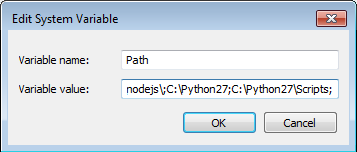
\includegraphics[width=1\textwidth]{figures/setting-env.png}}
		\caption{Gambar Setting Environment pip}
		\label{setting-env}
	\end{figure}
	
	\ref{setting-env}
	
	Harus sesuai dengan direktori hasil instalasi pip. Lalu untuk melakukan pengetesan dari berhasil atau tidak berhasilnya instalasi pip, dengan cara buka CMD lalu ketikkan perintah pip, maka akan muncul seperti gambar dibawah ini.
	
	\begin{figure} [ht]
		\centerline{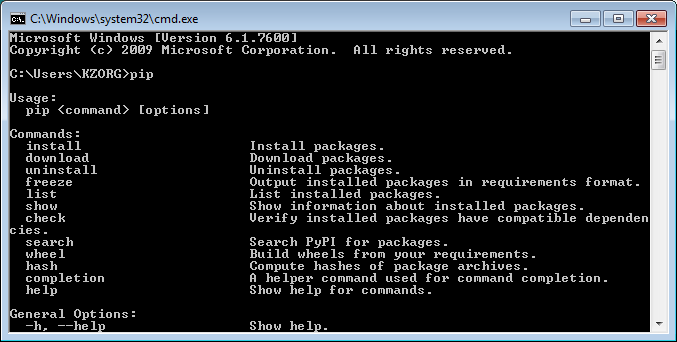
\includegraphics[width=1\textwidth]{figures/pip-terinstall.png}}
		\caption{Gambar pip yang Sudah Ter-install}
		\label{pip-terinstall}
	\end{figure}
	
	\ref{pip-terinstall}
				  
		\end{enumerate}

	\subsection{cara upgrade pip}
		\begin{item}
			\item python -m pip install -U pip
		\end{itemize}
		
	
	Dirangkum dari makalah \cite{feautrierpip}
	Dirangkum dari makalah \cite{nation2011qutip}
	Dirangkum dari artikel \cite{jewett2016moltemplate}
